% Errors

\only<1>{
\begin{minipage}{0.55\linewidth}
\centering
\[
\renewcommand{\arraystretch}{1}
\begin{array}{l}
\text{Block (Normal 3) } [ \\
\quad \colorbox{yellow!20}{$r(4) \leftarrow \phi[(0, \ \text{Normal 1}); \ (2, \ \text{Normal 2})];$} \\
\quad \colorbox{yellow!20}{$r(5) \leftarrow \phi[(1, \ \text{Normal 1}); \ (3, \ \text{Normal 2})]$} \\
] \ [ \\
\quad \colorbox{cyan!20}{$r(6) \leftarrow r(4) \times r(5);$} \\
\quad \colorbox{cyan!20}{$r(7) \leftarrow r(6) + i(1)$} \\
] \ ( \\
\quad \colorbox{red!20}{$\text{if } r(7) \leq i(100) \text{ then } \dots \text{ else } \dots$} \\
)
\end{array}
\]
\end{minipage}
\hfill
\begin{minipage}{0.40\linewidth}
\centering
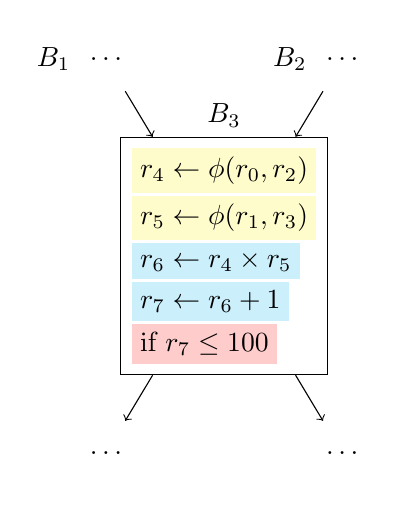
\begin{tikzpicture}
\node (b1) at (-1.5, 0) [minimum height=0.8cm, label=left:$B_1$] {$\dots$};
\node (b2) at (1.5, 0) [minimum height=0.8cm, label=left:$B_2$] {$\dots$};
\node (b3) at (0, -2.5) [draw, align=left, inner sep=4pt, label=above:$B_3$] {
    \colorbox{yellow!20}{$r_4 \leftarrow \phi(r_0, r_2)$} \\
    \colorbox{yellow!20}{$r_5 \leftarrow \phi(r_1, r_3)$} \\
    \colorbox{cyan!20}{$r_6 \leftarrow r_4 \times r_5$} \\
    \colorbox{cyan!20}{$r_7 \leftarrow r_6 + 1$} \\
    \colorbox{red!20}{if $r_7 \leq 100$}
};
\node (b4) at (-1.5, -5) [minimum height=0.8cm] {$\dots$};
\node (b5) at (1.5, -5) [minimum height=0.8cm] {$\dots$};

\draw[->] (b1) -- (b3);
\draw[->] (b2) -- (b3);
\draw[->] (b3) -- (b4);
\draw[->] (b3) -- (b5);
\end{tikzpicture}
\end{minipage}
}

\only<2>{
\centering
\begin{minipage}{0.55\linewidth}
\centering
\[
\renewcommand{\arraystretch}{1}
\begin{array}{l}
\text{Block (Normal 3) } [ \\
\quad \colorbox{yellow!20}{$r(\texttt{rdx}) \leftarrow \phi[(\texttt{rdx}, \ \text{Normal 1}); \ (\texttt{rdx}, \ \text{Normal 2})];$} \\
\quad \colorbox{yellow!20}{$r(\texttt{rbx}) \leftarrow \phi[(\texttt{rbx}, \ \text{Normal 1}); \ (\texttt{rbx}, \ \text{Normal 2})];$} \\
] \ [ \\
\quad \colorbox{cyan!20}{$r(\texttt{rbx}) \leftarrow r(\texttt{rdx}) \times r(\texttt{rbx});$} \\
\quad \colorbox{cyan!20}{$r(\texttt{rbx}) \leftarrow r(\texttt{rbx}) + i(1);$} \\
] \ ( \\
\quad \colorbox{red!20}{$\text{if } r(\texttt{rbx}) \leq i(100) \text{ then } \dots \text{ else } \dots$} \\
)
\end{array}
\]
\end{minipage}
\hfill
\begin{minipage}{0.40\linewidth}
\centering
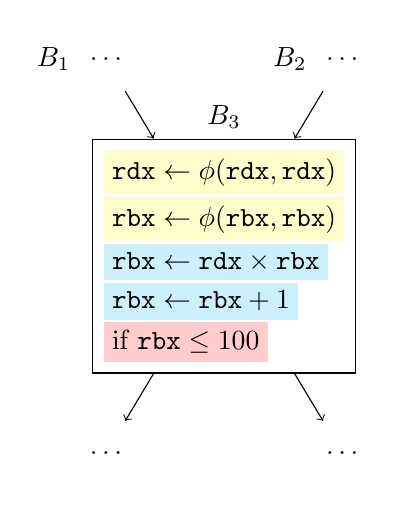
\begin{tikzpicture}
\node (b1) at (-1.5, 0) [minimum height=0.8cm, label=left:$B_1$] {$\dots$};
\node (b2) at (1.5, 0) [minimum height=0.8cm, label=left:$B_2$] {$\dots$};
\node (b3) at (0, -2.5) [draw, align=left, inner sep=4pt, label=above:$B_3$] {
    \colorbox{yellow!20}{$\texttt{rdx} \leftarrow \phi(\texttt{rdx}, \texttt{rdx})$} \\
    \colorbox{yellow!20}{$\texttt{rbx} \leftarrow \phi(\texttt{rbx}, \texttt{rbx})$} \\
    \colorbox{cyan!20}{$\texttt{rbx} \leftarrow \texttt{rdx} \times \texttt{rbx}$} \\
    \colorbox{cyan!20}{$\texttt{rbx} \leftarrow \texttt{rbx} + 1$} \\
    \colorbox{red!20}{if $\texttt{rbx} \leq 100$}
};
\node (b4) at (-1.5, -5) [minimum height=0.8cm] {$\dots$};
\node (b5) at (1.5, -5) [minimum height=0.8cm] {$\dots$};

\draw[->] (b1) -- (b3);
\draw[->] (b2) -- (b3);
\draw[->] (b3) -- (b4);
\draw[->] (b3) -- (b5);
\end{tikzpicture}
\end{minipage}
}

% \only<1>{
% \begin{align*}
% \nt{label} &::= \text{Normal} \ \mathbb N \mid \text{Point1} \ \mathbb N \mid \text{Point2} \ \mathbb N
% \\
% \nt{value} &::= i( \mathbb Z ) \mid r( \nt{register} ) \mid p( \mathbb N )
% \\
% \nt{expression} &::= \nt{value} \\
% &\mid \text{load} \ \nt{value} \\
% &\mid r( \nt{register} ) \makebox[1em]{+} \nt{value} \\
% &\mid r( \nt{register} ) \makebox[1em]{-} \nt{value} \\
% &\mid r( \nt{register} ) \makebox[1em]{*} \nt{value} \\
% &\mid r( \nt{register} ) \makebox[1em]{/} \nt{value}
% \\
% \nt{instruction} &::= r( \nt{register} ) \leftarrow \nt{expression} \\
% &\mid \text{store} \ r( \nt{register} ) \ r( \nt{register} )
% \\
% \nt{instructions} &::= \nt{instruction} ; \ \nt{instructions} \mid \nt{instruction}
% \\
% \nt{instructions-or-nil} &::= [ \nt{instructions} ] \mid []
% \end{align*}
% }

% \only<2>{
% \begin{align*}
% \nt{phi-arguments} &::= ( \nt{register} , \ \nt{label} ) ; \ \nt{phi-arguments} \\
% &\mid (\nt{register} , \ \nt{label})
% \\
% \nt{phi} &::= r( \nt{register} ) \leftarrow \phi \ \nt{phi-arguments-or-nil}
% \\
% \nt{phis} &::= \nt{phi} ; \ \nt{phis}
% \\
% \nt{phis-or-nil} &::= [ \nt{phis} ] \mid []
% \end{align*}
% }

% \only<3>{
% \begin{align*}
% \nt{condition} &::= r(\nt{register}) = \nt{val} \\
% &\mid r(\nt{register}) \neq \nt{val} \\
% &\mid r(\nt{register}) < \nt{val} \\
% &\mid r(\nt{register}) \leq \nt{val} \\
% &\mid r(\nt{register}) > \nt{val} \\
% &\mid r(\nt{register}) \geq \nt{val}
% \\
% \nt{jump-instruction} &::= \text{if} \ \nt{condition} \ \text{then} \ \nt{block} \ \text{else} \ \nt{block} \\
% &\mid \text{jump} \ \nt{block} \\
% &\mid \text{ret} \ r( \nt{register} )
% \\
% \nt{block} &::= \text{Block} \ ( \nt{label} ) \ \nt{phis-or-nil} \ \nt{instructions-or-nil} \ ( \nt{jump-instruction} )
% \end{align*}
% }